% BOTTOM caption
% ------------------------
\begin{figure}[!htbp]
\centering
\vspace{1\baselineskip}
% ------------------------
%
% Main information
% ===========================================================
\begin{subfigure}{0.49\textwidth}
	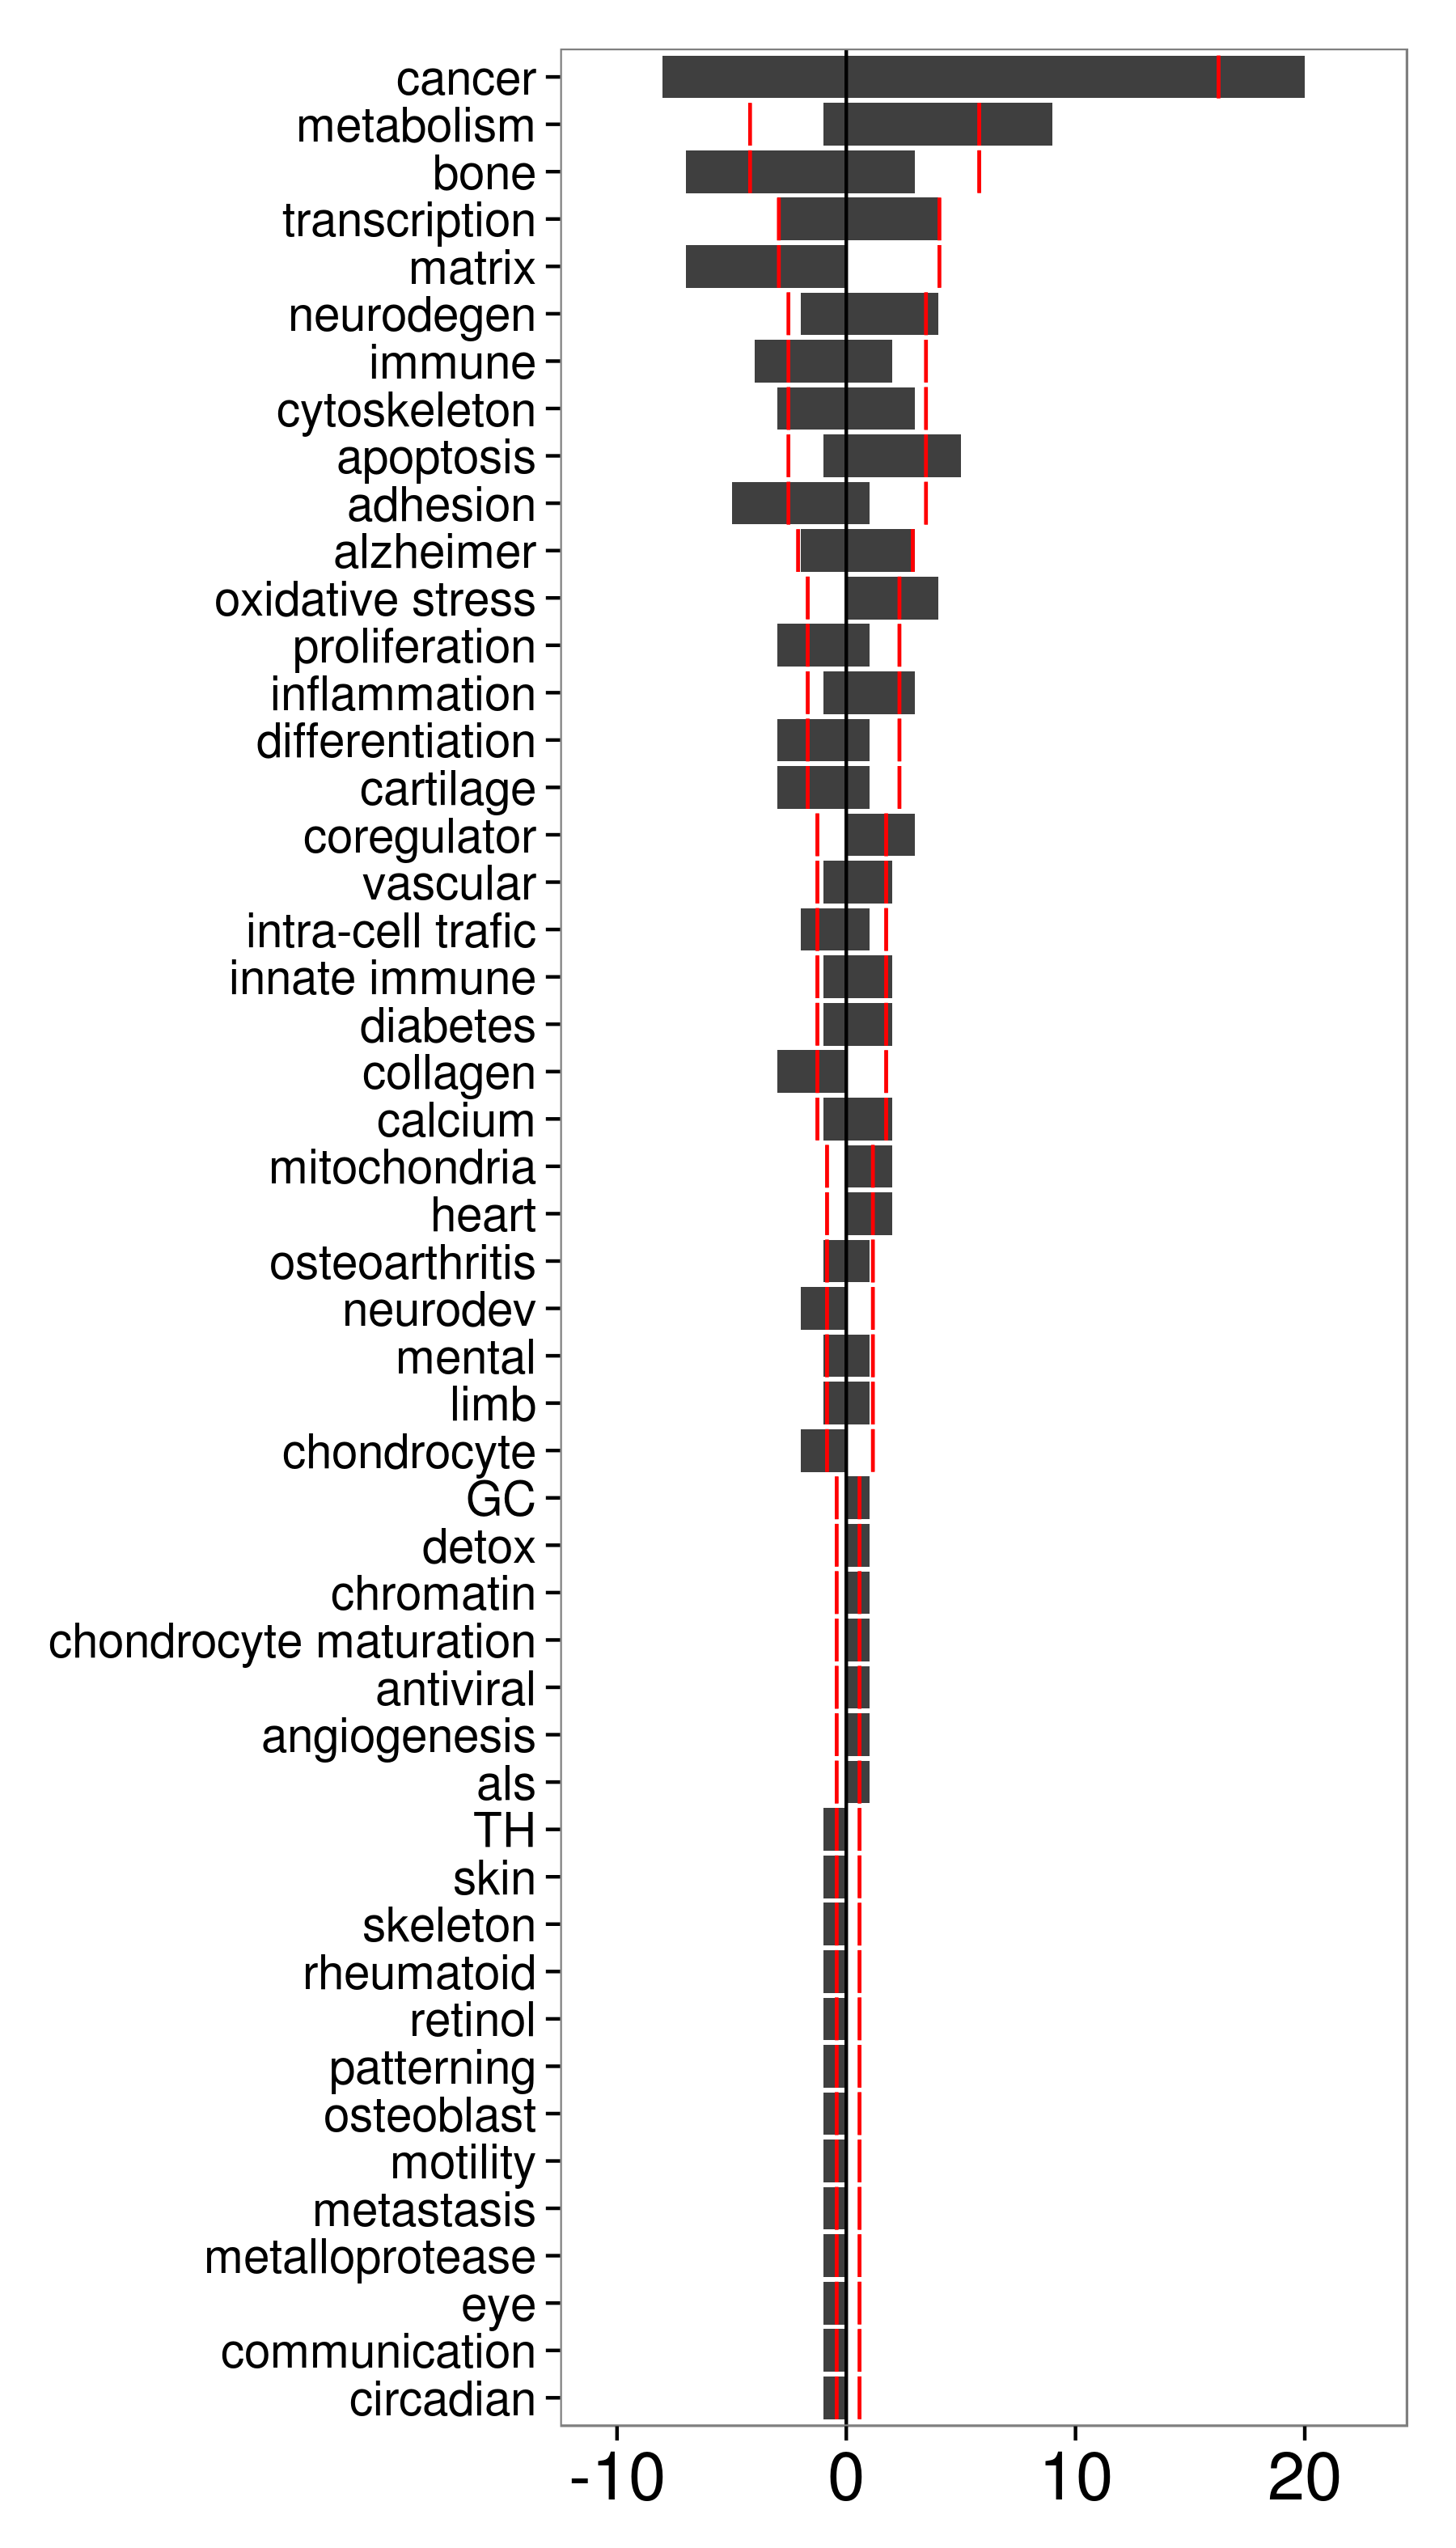
\includegraphics[width=\textwidth]
	{Figures/tfc-manualannot-antago/tfc-manualannot-antago-c.png}
	\caption{}
	\label{subfig:tfc-manualannot-antago-c}
\end{subfigure}
\begin{subfigure}{0.49\textwidth}
	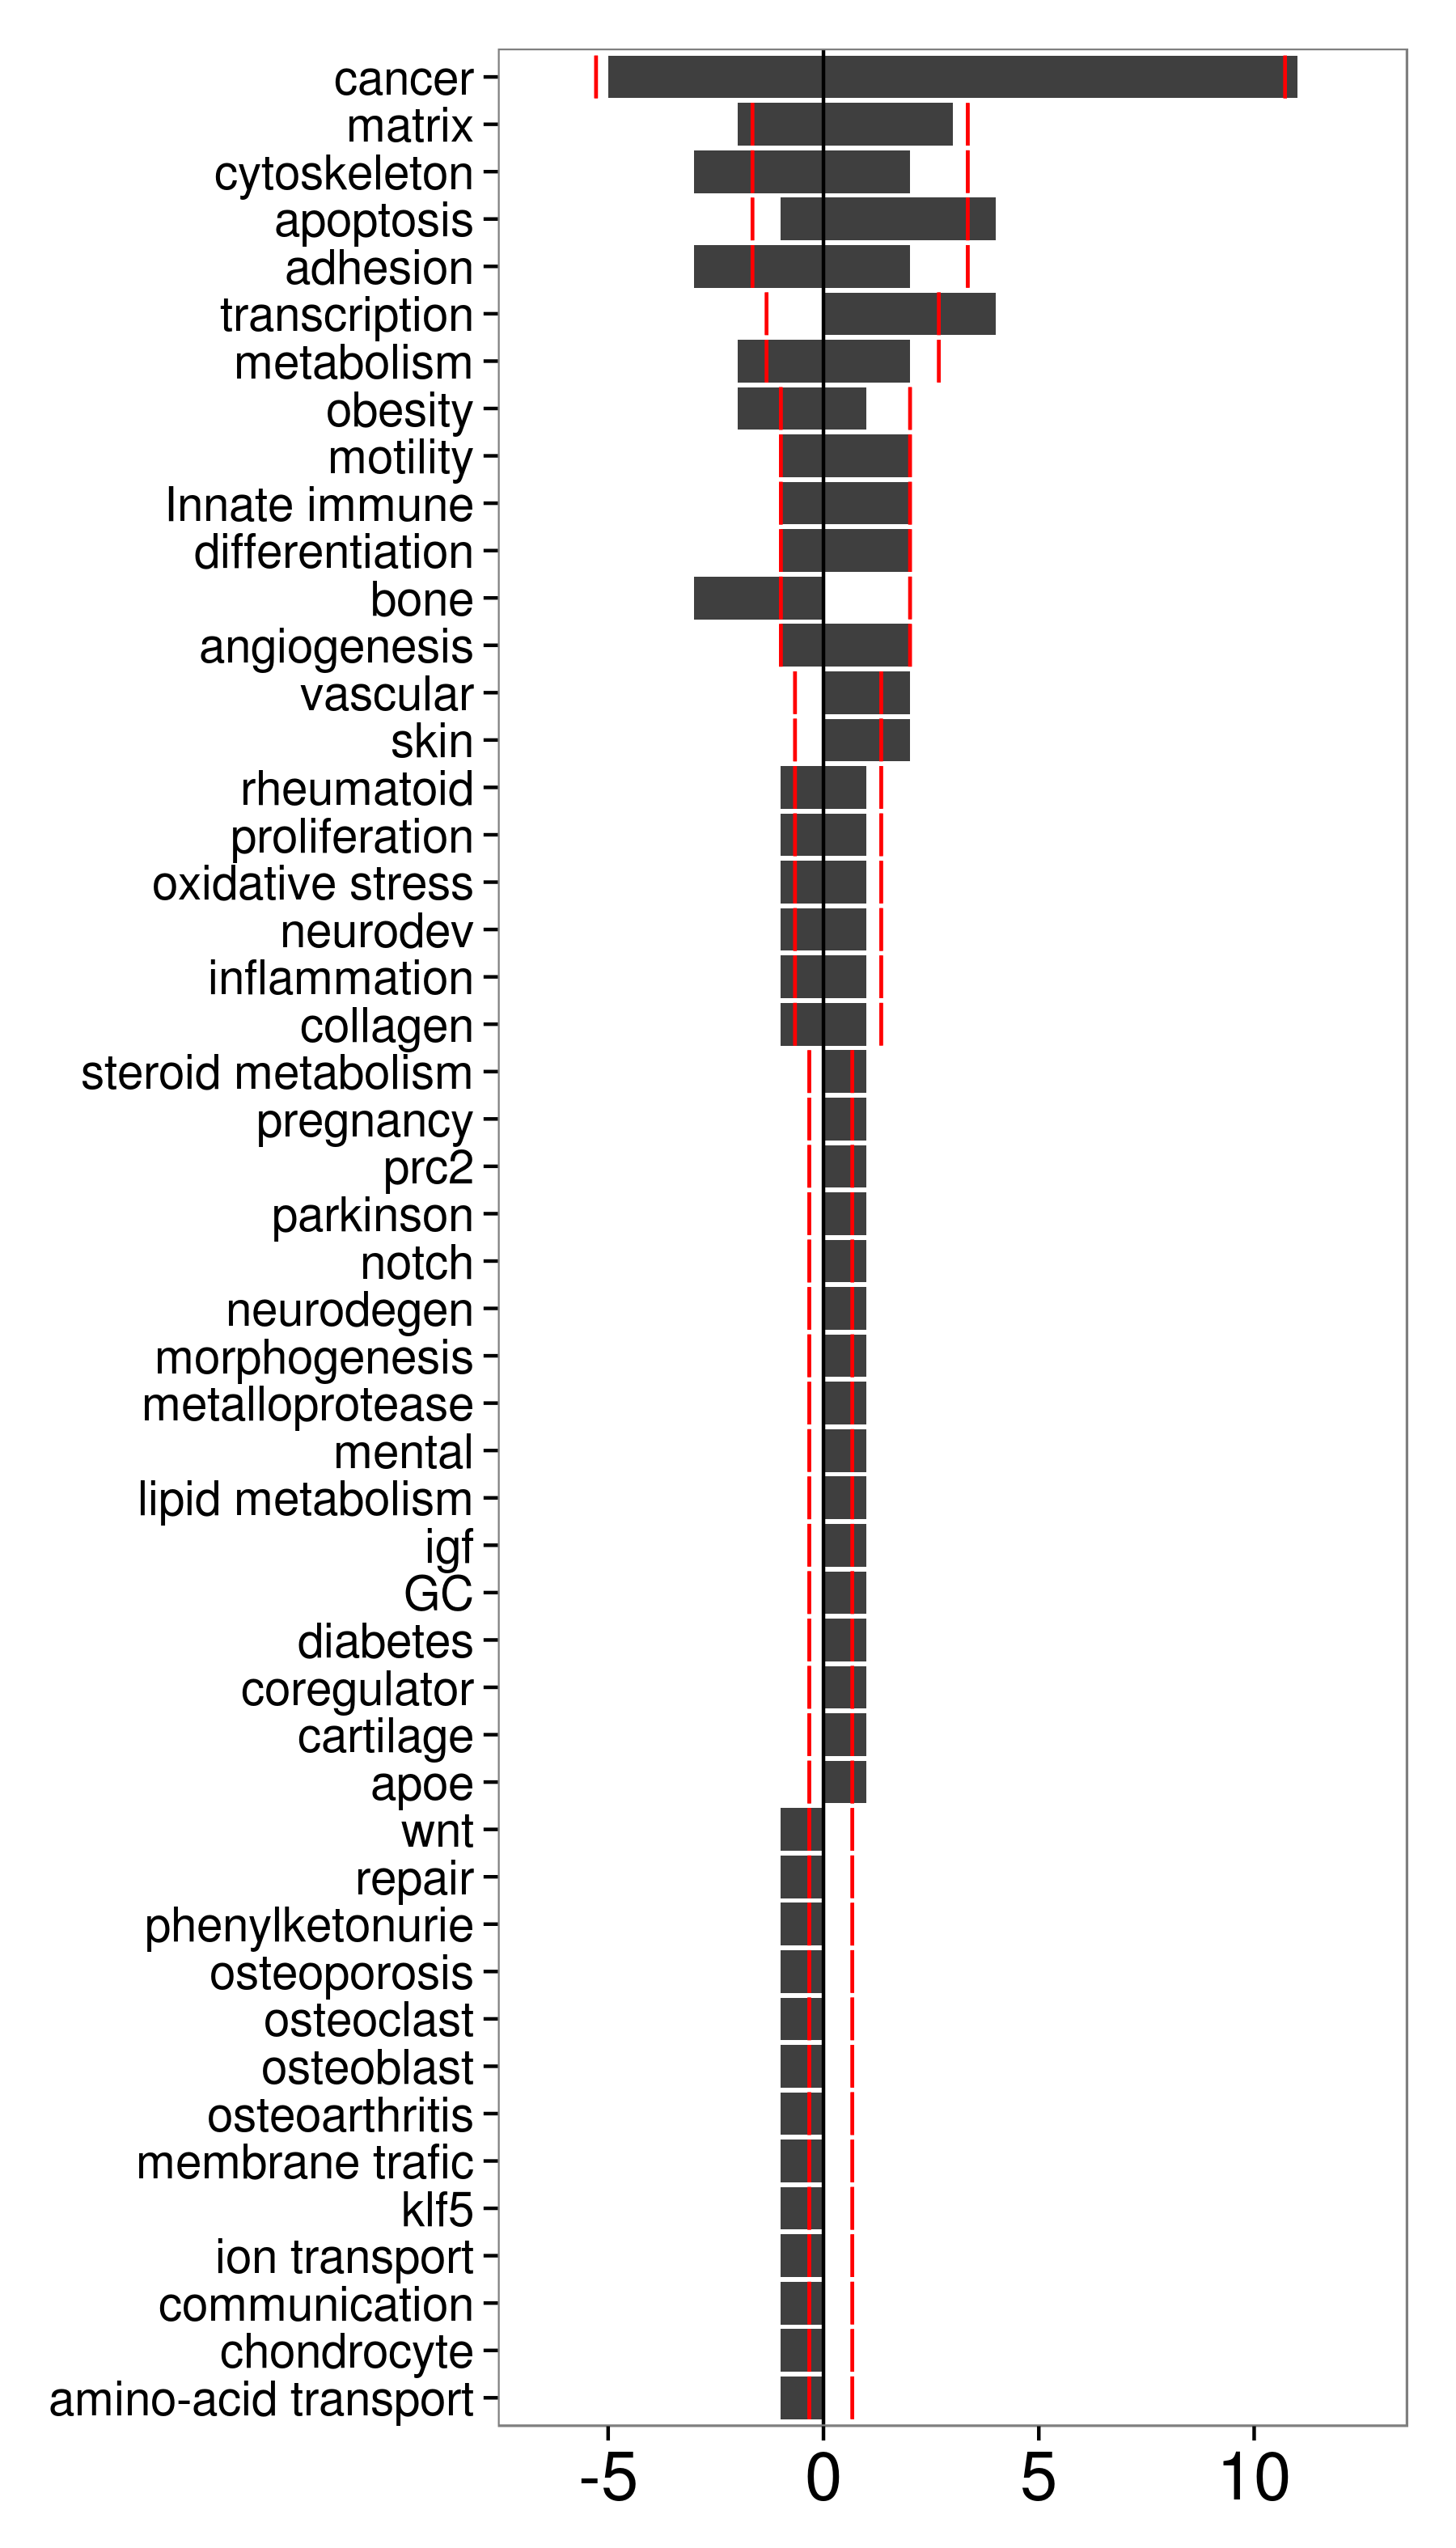
\includegraphics[width=\textwidth]
	{Figures/tfc-manualannot-antago/tfc-manualannot-antago-t.png}
	\caption{}
	\label{subfig:tfc-manualannot-antago-t}
\end{subfigure}
\caption[Catégories fonctionnelles enrichies parmi les gènes ``antagonisés'' dans l'épiderme caudal]
{
Catégories fonctionnelles enrichies parmi les gènes présentant un profil de type ``antagonisme'' et réprimés (valeurs négatives, partie gauche de chaque sous-figure) ou induits (valeurs positives, partie droite de chaque sous-figure) dans l'épiderme caudal.
\ref{subfig:tfc-manualannot-antago-c} Effets de la \gls{cort} antagonisés par la \gls{t3}, correspondant aux clusters 1-4 de la \autoref{fig:tfc-clusters-antago}~A.
\ref{subfig:tfc-manualannot-antago-t} Effets de la \gls{t3} antagonisés par la \gls{cort}, correspondant aux clusters 5-6 de la \autoref{fig:tfc-clusters-antago}~B.
La valeur absolue de l'axe des abscisses représente le nombre de gènes associé à chaque terme (axe des ordonnées).
Seuls les 50 termes les plus représenté sont illustrés ici.
Les barres verticales rouges correspondent au nombre théorique de gènes associés à chaque terme dans le cas d'une répartition aléatoire entre répression et induction.
}
\label{fig:tfc-manualannot-antago}
% ===========================================================
%
% BOTTOM caption
% ------------------------
\end{figure}
% ------------------------